\documentclass[11pt]{article}
\usepackage[margin=1in]{geometry}
\usepackage{amsmath,amssymb}
\usepackage[T1]{fontenc}
\usepackage{lmodern}
\usepackage{microtype}
\usepackage{booktabs}
\usepackage{graphicx}
\usepackage{xurl}
\usepackage{hyperref}
\hypersetup{colorlinks=true,linkcolor=blue,citecolor=blue,urlcolor=blue,
  pdftitle={Do players quit after a new personal-best rating? A pre-registered, placebo-controlled test on Lichess},pdfauthor={Qianghao Wu}}
\title{Do players quit after a new personal-best rating?\\ A pre-registered, placebo-controlled test on Lichess}
\author{Qianghao Wu}
\date{November 25, 2026}
\pagestyle{plain}
\begin{document}
\maketitle
\begin{abstract}
Anderson and Green (PNAS, 2018) found that blitz players on the Free Internet Chess Server (FICS) quit more often just after they set a new personal-best rating: the probability of quitting jumps by 4.5 percentage points (pp), or 20\%. We test the same claim on Lichess with public data. We rebuilt the rating history of every Lichess blitz player from the headers of all 45 million rated games of 2013--2015. Before we computed any quit rate, we fixed the sample, the estimator (local linear regression, triangular kernel, bandwidth 15 rating points, errors clustered by player), the controls and a decision rule. Among 10.8 million player-games after a win, with 37,391 new personal bests, the jump in the probability of quitting (no new game within 60 minutes) is $+0.51$~pp, 95\% confidence interval $-0.38$ to $+1.39$~pp, on a quit rate of 18.55\% just below the personal best. The interval contains zero, and its upper bound is below 4.5~pp. With the same estimator, a known reference point (ratings that cross a multiple of 100) gives $+2.83$~pp ($z=28.6$), and an added step of 4.5~pp is recovered. Placebo cutoffs and a within-player shuffle show no jump. In a second test, fixed before its data were downloaded, we used 2016, after the Lichess source code added a ``Highest rating'' display to its statistics pages. The jump is $+0.88$~pp ($+0.25$ to $+1.52$). This jump is small and not robust to all variants, and it is not significantly larger than in 2013--2015. The upper bounds of the two primary intervals, 1.39 and 1.52~pp, are about one third of the FICS value. The result is an association on one platform. It does not show that the FICS result is wrong.

This work has not yet been reviewed by experts. The computations and the text were produced by AI models (from Anthropic and OpenAI), working under the author's direction.
\end{abstract}
\medskip
\noindent\textbf{Keywords:} reference points, personal bests, quitting, regression discontinuity, online chess, Lichess, replication, pre-registration.

\section{Introduction}

\subsection{The claim}

A reference point is an outcome that a person compares other outcomes with. Results below it feel like losses, and results above it feel like gains. Anderson and Green~\cite{ag} proposed that a personal best, the best past performance of a person, acts as a reference point. They used 133 million blitz games from the Free Internet Chess Server (FICS), 2000--2015. Each player has a rating. The FICS user page shows the current rating and the best past rating. Players also ``receive text and sound notifications when they reach a new personal best''~\cite{ag}.

Their unit is the player-game: one player in one game. Their running variable is ``the distance between a player's current rating and her personal best rating from before her last game''~\cite{ag}. They define quitting as ``not playing another game within 1 h of finishing the most recent game''~\cite{ag}. For player-games that follow a win, they report:

\begin{quote}
``The probability of quitting jumps across the reference point---a 4.5 percentage point, or 20\%, increase. As predicted, players are discontinuously more likely to quit after setting a new personal best.''~\cite{ag}
\end{quote}

The same paper reports a second effect: ``At the reference point, performance is $\sim$1 percentage point higher than if the prevailing trend had continued unabated''~\cite{ag}. We do not test this effort effect. This paper tests only the quitting jump.

The evidence in~\cite{ag} comes from one platform, and on that platform the personal best is very visible. We ask if the same jump occurs on a second large platform, Lichess, where the data are public.

\subsection{Main result}

\begin{quote}
\textbf{Result.} On Lichess blitz, 2013--2015, the jump in the probability of quitting at a new personal best is $+0.51$~pp (standard error 0.45; 95\% CI $-0.38$ to $+1.39$~pp), on a quit rate of 18.55\% just below the personal best. Under the rule that we fixed in advance, the outcome is \emph{null, smaller than FICS}: the interval contains 0, and its upper bound is below the FICS value of 4.5~pp.
\end{quote}

The same estimator detects a known reference point in the same data (ratings that cross a multiple of 100: $+2.83$~pp, $z=28.6$). In 2016, after the Lichess source code added a display of the highest rating to a statistics page, the jump is $+0.88$~pp (95\% CI $+0.25$ to $+1.52$). It is small, it is not robust to all variants, and it is not significantly larger than the 2013--2015 jump (Section~\ref{sec:2016}).

\subsection{Earlier work}

On 2026-11-24, and again on 2026-11-25, we searched for work that cites~\cite{ag} (36 works in Semantic Scholar, 40 in OpenAlex), arXiv, Zenodo, GitHub, the Lichess bibliography of research papers and general web search. We found no other test of the personal-best quitting jump on Lichess. The closest work is the following.

\begin{itemize}
\item González-Díaz, Palacios-Huerta and Abuín~\cite{gonzalez} study personal bests as reference points in official over-the-board chess (FIDE ratings) and compare men and women. Their data are not online games.
\item Kurashima and co-authors~\cite{kurashima} study personal history as a reference point on Codeforces, a competitive-programming site.
\item Avoyan, Khubulashvili and Mekerishvili~\cite{avoyan, avoyanssrn} study when players on an online chess platform stop a session after wins and losses. They do not test a discontinuity at the personal best.
\item Krumer, Otto and Pawlowski~\cite{krumer} study how the salience of a reference point changes behavior, with data from ski jumping.
\item Bobev~\cite{bobev} posted a Lichess study of session ending at round-number ratings (1200 to 2100) on Zenodo on 2026-11-03. The record was deleted on 2026-11-09 with the reason ``retracted''. Its manuscript does not mention personal bests. Its topic overlaps with our round-number control, not with our main test.
\end{itemize}

Anderson and Green also report a round-number effect on FICS: ``players with ratings ending in 01 quit 3.5 percentage points more often than players with ratings ending in 99''~\cite{ag}. We use a version of this effect as a positive control (Section~\ref{sec:controls}).

\section{Data}

The Lichess open database~\cite{lichessdb} publishes every rated standard game of each month as a PGN file, under the CC0 license. We used the 36 files from 2013-01 to 2015-12 (45,043,493 games, 90,085,152 player-games) and, for Section~\ref{sec:2016}, the 12 files of 2016. Each file was checked against the published SHA-256 list. We kept only these header tags: \texttt{Event}, \texttt{Site}, \texttt{White}, \texttt{Black}, \texttt{Result}, \texttt{UTCDate}, \texttt{UTCTime}, \texttt{WhiteElo}, \texttt{BlackElo}, \texttt{WhiteRatingDiff}, \texttt{BlackRatingDiff}, \texttt{TimeControl} and \texttt{Termination}. The speed (bullet, blitz, classical, correspondence) comes from \texttt{Event}. In this period Lichess kept a separate rating for each speed.

The files contain only rated games of standard chess. The headers have no end time, no rating deviation and no flag for computer accounts. In 2013--2015, 447,358 player-games (0.5\%) have no \texttt{RatingDiff} tag. For these, the post-game rating is the pre-game rating of the next game at the same speed.

\section{Method}\label{sec:method}

\paragraph{Pre-registration.} The protocol (\texttt{PROTOCOL.md}) was committed on 2026-11-25 at 03:00 CET, before any quit rate was computed. The first outcome file was committed 13 minutes later. The commit order is the evidence; it cannot prove that no quit rate was computed on part of the data before 03:00. Before the protocol, we only looked at the header format, at how well consecutive ratings agree, and at the start rating of new players. Two addenda were written later, and each states what had been seen before it: addendum A (Section~\ref{sec:2016}) and addendum B (exclusion of 917 rated games in which one account played both sides; the primary numbers are identical with and without them).

\paragraph{Definitions.} For player $i$ and blitz game $t$, $r_t$ is the rating after the game: the pre-game rating plus \texttt{RatingDiff}. The personal best $\mathrm{PB}_t$ is the maximum of $r_s$ over all earlier blitz games $s$ of the player. The running variable is $x_t = r_t - \mathrm{PB}_t$, in integer rating points; $x_t \ge 1$ is a new personal best. The header gives the start time and the time control (base $b$ seconds, increment $k$). We estimate the end of the game as at most $D_t = 2(b + 40k)$ seconds after the start. Then $\mathrm{quit}_t = 1$ if the next rated game of the player, at any speed, starts more than $60\,\mathrm{min} + D_t$ after the start of game $t$, or if there is no next game.

\paragraph{Sample.} A player-game is in the primary sample if all of these are true: (1) it is blitz; (2) the player's first blitz game in the data has the Lichess start rating 1500, so the history is complete; (3) it is the player's 200th blitz game or later; (4) the player set no new personal best in the previous 20 blitz games; (5) the player won the game; (6) the previous blitz game started at most 30 days earlier; (7) the game started on or before 2015-12-30 23:59:59 UTC. Rules 3--5 follow~\cite{ag}. Rule 6 replaces their filter on rating deviation, which the headers do not give. Rule 7 keeps a window after each kept game inside the data. The last game of the 2015-12 file starts at 2015-12-31 22:59:57 UTC, so this window is 23 hours, not the 24 hours that the protocol states. This has no effect on the 60-minute outcome. The sample has 10,755,282 player-games of 26,722 players, with 37,391 new personal bests.

\paragraph{Estimator.} We fit a local linear regression of quit on $c = x - 0.5$, with separate slopes on each side of $c=0$, a triangular kernel and a bandwidth of $h = 15$ rating points ($x$ from $-14$ to $15$). The jump is the coefficient of $\mathbf 1[x \ge 1]$. Standard errors are clustered by player, and the 95\% CI is the estimate $\pm 1.96$ standard errors. The relative jump is the jump divided by the fitted value just below the cutoff (the left limit). We chose this estimator and bandwidth ourselves. The main text of~\cite{ag} does not give the estimator or the bandwidth for the 4.5~pp value. We did not read its supplementary information, so we do not know the FICS estimator.

\paragraph{Decision rule.} From the primary 95\% CI: \emph{supported} if the lower bound is above 0; \emph{opposite sign} if the upper bound is below 0; \emph{null, smaller than FICS} if the interval contains 0 and the upper bound is below 4.5~pp; \emph{inconclusive} if the interval contains 0 and the upper bound is 4.5~pp or more. If the upper bound is below 4.5~pp, the FICS magnitude is rejected.

\paragraph{Controls.}\label{sec:controls} All were fixed in the protocol.
\begin{enumerate}
\item Placebo cutoffs at PB$-50$, PB$-35$, PB$-25$ (data with $x\le 0$ only) and PB$+10$ (data with $x \ge 1$ only).
\item Covariate balance: the same regression with each of four covariates as the dependent variable: the rating gain of the game, the opponent rating minus the own rating, the log of the minutes since the previous game, and the log of the game index. These are fixed before the decision to quit.
\item A within-player shuffle of the quit labels in the bandwidth sample, 200 permutations.
\item An injected jump: in a copy of the data, quit is set to 1 at random to the right of the cutoff, so that the right-side quit rate rises by 4.5~pp in expectation.
\item A round-number control: the same estimator, with the running variable $d = ((r+50) \bmod 100) - 50$ and the cutoff between ratings that end in 99 and 00. This control uses rules 1--3 and 5--7, without the personal-best filter. It differs from the FICS statistic in two ways. Anderson and Green compare ratings that end in 01 with ratings that end in 99, and put 00 at the cutoff; we put 00 on the right side. Our control uses only player-games after a win.
\end{enumerate}

\section{Results}\label{sec:results}

\begin{figure}[t]
\centering
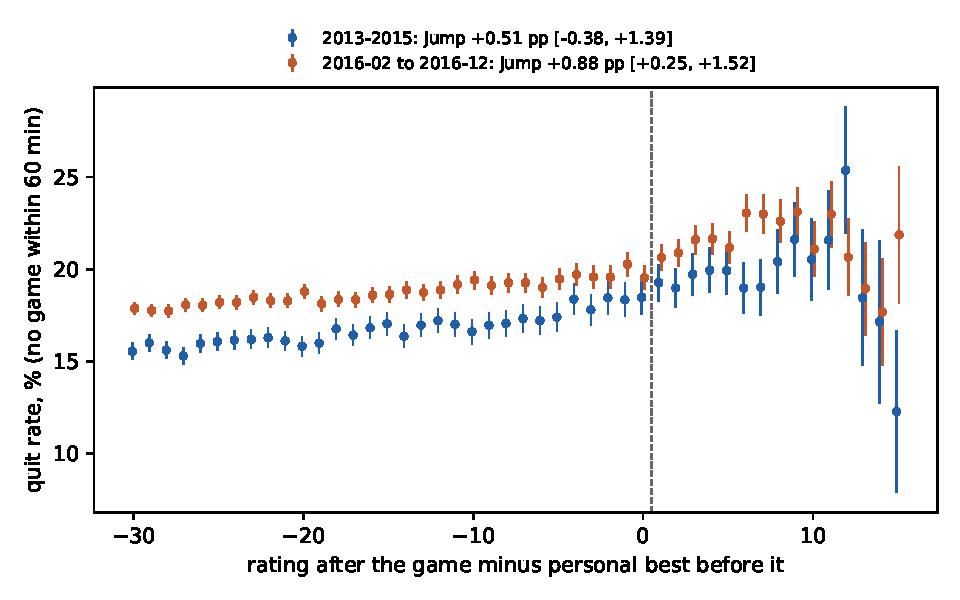
\includegraphics[width=0.85\linewidth]{fig_quit_pb.pdf}
\caption{Blitz quit rate (no new game within 60 minutes) by the rating after a won game minus the personal best before it. Blue: 2013--2015 (primary). Orange: 2016-02 to 2016-12 (Section~\ref{sec:2016}). The dashed line is the cutoff between $x=0$ and $x=1$. Error bars are 95\% binomial intervals of each bin, without clustering by player. The legend gives the local linear estimate of the jump and its 95\% CI.}
\label{fig:main}
\end{figure}

Figure~\ref{fig:main} shows the quit rate by distance to the personal best. In 2013--2015 the quit rate rises slowly from about 15.5\% at $x=-30$ to about 18.5\% at $x=0$. Above the personal best it rises faster, in both periods. The local linear fit allows a different slope on each side, so this change of slope does not count as a jump. We see no step at the cutoff that is larger than the noise.

\begin{table}[h]
\centering
\small
\begin{tabular}{lrrp{6.3cm}}
\toprule
Estimate (2013--2015 blitz) & Jump, pp & SE & Note \\
\midrule
\textbf{Primary} ($h=15$) & $\mathbf{+0.51}$ & 0.45 & 95\% CI $[-0.38, +1.39]$; left limit 18.55\%; $n = 185{,}385$ (14,903 players) \\
Relative jump & $+2.7\%$ & & FICS: $+20\%$ \\
Minimum detectable effect (80\% power) & 1.26 & & $2.8 \times$ SE \\
\midrule
Round-number control & $+2.83$ & 0.10 & $z = 28.6$; relative $+23.5\%$; $n = 3{,}406{,}437$ \\
Injected 4.5~pp step & $+5.17$ & 0.48 & returned addition $+4.66$~pp \\
Placebo PB$-50$ & $-0.04$ & 0.15 & $z=-0.26$ \\
Placebo PB$-35$ & $+0.09$ & 0.18 & $z=0.48$ \\
Placebo PB$-25$ & $+0.13$ & 0.20 & $z=0.62$ \\
Placebo PB$+10$ & $+2.45$ & 1.31 & $z=1.88$ \\
Within-player shuffle & & & mean $+0.24$, SD 0.38; $p=0.28$ \\
\bottomrule
\end{tabular}
\caption{Primary estimate and controls for 2013--2015. Source: \texttt{data/results.json}.}
\label{tab:main}
\end{table}

\paragraph{Primary test.} Table~\ref{tab:main} gives the primary estimate. The jump is $+0.51$~pp with a 95\% CI from $-0.38$ to $+1.39$~pp. The decision is \emph{null, smaller than FICS}. The relative jump is $+2.7\%$; the FICS value is $+20\%$. A model-free comparison of the two bins next to the cutoff gives 18.46\% at $x=0$ and 19.27\% at $x=1$, a difference of $+0.81$~pp (SE 0.69).

\paragraph{Controls.} The round-number control gives $+2.83$~pp ($z=28.6$), a relative jump of $+23.5\%$. So the method finds a known reference point in the same data. The bins show a clear step at the hundred: 12.07\% at ratings that end in 99 and 14.58\% at ratings that end in 00. The control is not constant in time. By year, it is $+0.38$~pp (SE 0.39) in 2013, $+1.54$ (0.17) in 2014 and $+3.42$ (0.12) in 2015 (independent check, \texttt{checks/independent/extra\_2013\_2015.log}). The pooled value comes mostly from 2014 and 2015, which also hold most of the primary sample.

When we add a step of 4.5~pp to the data, the estimator returns $+5.17$~pp, that is, $+4.66$~pp more than the primary estimate. This control is mechanical: it shows that the estimator returns a step of 4.5~pp when one is added to the data. It does not show that the personal best is measured correctly; Section~\ref{sec:checks} treats that question. The three placebo cutoffs below the personal best show no jump. The placebo at PB$+10$ gives $+2.45$~pp ($z=1.88$), which is not significant at 5\%; above the personal best the data are few and the slope is steep. The within-player shuffle gives $p=0.28$. Its mean is $+0.24$~pp, not 0, because the shuffle keeps the differences between players.

\paragraph{Covariate balance.} Three of four covariates are not balanced at the cutoff. Players who just set a new personal best won a slightly smaller rating gain ($-0.29$ points, $z=-2.37$), against relatively weaker opponents (opponent minus own rating $-13.9$ points, $z=-4.38$), and had played more games (log game index $+0.054$, $z=3.74$). The time since the previous game is balanced ($z=0.44$). With the rating gain as a covariate, the jump is $+0.54$~pp (SE 0.45). With the gain, the opponent rating difference and the log game index as covariates, it is $+0.65$~pp (0.46). With player fixed effects, it is $+0.24$~pp (0.44).

\begin{table}[h]
\centering
\small
\begin{tabular}{lrr}
\toprule
Variant (2013--2015, not part of the decision) & Jump, pp & SE \\
\midrule
Quit = no new game within 24 h (left limit 3.84\%) & $+0.12$ & 0.22 \\
Quit = next start more than 90 min after this start & $+0.54$ & 0.44 \\
Bandwidth $h = 10$ & $+0.49$ & 0.53 \\
Bandwidth $h = 25$ & $+0.92$ & 0.39 \\
Without tournament games & $+0.52$ & 0.52 \\
Rating gain as a covariate & $+0.54$ & 0.45 \\
Bullet & $+0.53$ & 0.37 \\
Classical & $+0.19$ & 0.65 \\
Adjacent bins, $x=0$ versus $x=1$ & $+0.81$ & 0.69 \\
\bottomrule
\end{tabular}
\caption{Pre-registered robustness variants, 2013--2015. Source: \texttt{data/results.json}.}
\label{tab:rob}
\end{table}

\paragraph{Robustness.} Table~\ref{tab:rob} gives the pre-registered variants. Only $h=25$ gives a CI that excludes 0 ($+0.92$~pp, $z=2.38$). Its point estimate is about one fifth of the FICS jump. In all variants, the upper bound of the 95\% CI is below 4.5~pp. The largest upper bound is 2.17~pp (adjacent bins).

\section{Second period: 2016, after a ``Highest rating'' display}\label{sec:2016}

FICS shows the personal best and announces a new one. We found no display of the personal best on Lichess in 2013--2015, but we did not confirm that none existed. In the Lichess source code, commit \texttt{5e9fde4a} (2015-12-26) adds a ``Highest rating'' panel to the statistics page of each speed, and commit \texttt{4dacb459} (2016-01-10) links it from the user page~\cite{lila}. We did not confirm the date when this change went live on lichess.org. If the personal best matters only when it is visible, we expect a larger jump after the change.

After we saw the 2013--2015 result, and before we downloaded any 2016 file, we added this test to the protocol (addendum A). Period B is blitz games from 2016-02-01 to 2016-12-30, with histories from 2013-01. Period A is 2013--2015 from the same build. The difference B$-$A has the standard error $\sqrt{\mathrm{SE}_A^2 + \mathrm{SE}_B^2}$. This treats the periods as independent; many players are in both, so it is an approximation.

\begin{table}[h]
\centering
\small
\begin{tabular}{lrrp{5.6cm}}
\toprule
Period & Jump, pp (SE) & 95\% CI & Note \\
\midrule
A: 2013-01 to 2015-12 & $+0.51$ (0.45) & $[-0.38, +1.39]$ & left limit 18.55\%; $n=185{,}385$ \\
B: 2016-02 to 2016-12 & $+0.88$ (0.32) & $[+0.25, +1.52]$ & left limit 19.86\%; $n=407{,}350$ (37,708 players) \\
B $-$ A & $+0.37$ (0.55) & $[-0.71, +1.46]$ & salience prediction not supported \\
\bottomrule
\end{tabular}
\caption{Addendum A. Source: \texttt{data/addendum/addendum.json}.}
\label{tab:2016}
\end{table}

\begin{table}[h]
\centering
\small
\begin{tabular}{lrrr}
\toprule
Period B variant & Jump, pp & SE & $z$ \\
\midrule
Primary ($h=15$) & $+0.88$ & 0.32 & 2.73 \\
Bandwidth $h = 10$ & $+0.59$ & 0.39 & 1.49 \\
Bandwidth $h = 25$ & $+1.18$ & 0.27 & 4.34 \\
Quit = no new game within 24 h & $+0.19$ & 0.15 & 1.28 \\
Quit = next start more than 90 min after this start & $+0.94$ & 0.32 & 2.97 \\
Without tournament games & $+0.86$ & 0.36 & 2.39 \\
Rating gain as a covariate & $+0.90$ & 0.33 & 2.77 \\
Bullet & $+1.48$ & 0.37 & 3.99 \\
Classical & $+1.11$ & 0.43 & 2.59 \\
Adjacent bins, $x=0$ versus $x=1$ & $+1.11$ & 0.49 & 2.27 \\
\midrule
Placebo PB$-50$ & $-0.27$ & 0.11 & $-2.51$ \\
Placebo PB$-35$ & $-0.08$ & 0.13 & $-0.66$ \\
Placebo PB$-25$ & $+0.16$ & 0.15 & 1.07 \\
Placebo PB$+10$ & $-0.50$ & 0.87 & $-0.57$ \\
Round-number control & $+3.46$ & 0.07 & 47.86 \\
Injected 4.5~pp step & $+5.53$ & 0.34 & 16.38 \\
\bottomrule
\end{tabular}
\caption{All period B estimates. Source: \texttt{data/addendum/period\_B.json}.}
\label{tab:2016rob}
\end{table}

Tables~\ref{tab:2016} and~\ref{tab:2016rob} give the results. In period B, the jump is $+0.88$~pp, or $+4.4\%$ relative. Under the decision rule, the label of this result is \emph{supported}, and the FICS magnitude is again outside the CI. The evidence for this small jump is weak. With $h=10$ the jump is $+0.59$~pp ($z=1.49$), and with the 24-hour outcome it is $+0.19$~pp ($z=1.28$); neither is significant. The placebo at PB$-50$ fails ($-0.27$~pp, $z=-2.51$). In the within-player shuffle, none of the 200 permutations is as large as the observed jump ($p<0.005$). The covariates have the same imbalance as in period A (gain $z=-4.38$, opponent rating difference $z=-3.44$, log game index $z=3.39$). The difference B$-$A is $+0.37$~pp, with a 95\% CI from $-0.71$ to $+1.46$~pp. So the data do not show that the jump grew when the personal best became visible.

\section{How the result was checked}\label{sec:checks}

\paragraph{Rerun from the raw data.} The script \texttt{checks/rerun.py} downloads the 48 monthly files (about 22~GB, streamed and not stored), checks every SHA-256 against the published list, builds the tables, runs the analysis and compares every number with \texttt{data/expected.json} at a relative tolerance of $10^{-9}$. It passed from a fresh clone during the study (44 minutes) and again from a second clean clone during verification (about 53 minutes): 48 checksums matched, and 0 numbers differed.

\paragraph{Independent implementation.} A second agent wrote its own pipeline before it read the main code in detail (\texttt{checks/independent/}). It reads the games in time order and keeps the state of each player in plain Python, and it fits the regression with \texttt{statsmodels} and with a second numpy implementation. It gives the same counts (90,085,152 player-games, 917 self-play games, 10,755,282 player-games after the personal-best filter, 37,391 new personal bests, 26,722 players) and the same estimates to four decimals: $+0.5083$~pp (SE 0.4509) for the primary jump, $+0.8833$~pp (SE 0.3235) for period B, and $+2.8344$~pp for the round-number control.

\paragraph{Is the null caused by a wrong personal best?} An error in the rating history would make the personal best wrong and would weaken a real jump. On a 1-in-50 sample of consecutive blitz games of one player, the next pre-game rating equals $r_t$ exactly in 96.1\% of cases in 2013, 95.5\% in 2014 and 98.5\% in 2015. In 3.4\%, 4.1\% and 1.3\% of cases, the difference is more than 5 points. We did not find the cause. Three variants of the definitions give the same result: the personal best as the maximum of all earlier pre-game and post-game ratings ($+0.46$~pp, SE 0.47); the post-game rating as the pre-game rating of the next blitz game ($+0.52$~pp, SE 0.45); and only rows where the next pre-game rating confirms $r_t$ ($+0.56$~pp, SE 0.45). In all three, the upper bound of the 95\% CI is below 1.5~pp. The round-number bins (12.07\% at 99, 14.58\% at 00) also show that $r_t$ is correct to the rating point in most rows.

\section{Limits}\label{sec:limits}

\begin{enumerate}
\item The result is an association. The covariate imbalance shows that player-games just above and just below the personal best are not fully comparable.
\item The comparison value 4.5~pp is the number in the main text of~\cite{ag}. We do not know the estimator that gave it, because we did not read the supplementary information. Our estimator was fixed in advance, and the model-free adjacent-bin difference ($+0.81$~pp, SE 0.69) is also far below 4.5~pp.
\item Anderson and Green excluded computer accounts. The Lichess headers of 2013--2016 have no flag for computer accounts or cheaters, so we did not exclude them.
\item The headers have no end time. The 60-minute rule uses an upper estimate of the game length. A start-to-start rule gives the same result.
\item The files hold only rated standard games. A player who switches to casual or variant games counts as quitting.
\item The headers have no rating deviation. A 30-day inactivity filter replaces the FICS filter on rating deviation.
\item Histories start in 2013-01. The start-rating rule removes most accounts that played before. An account that played blitz before 2013 and still had the rating 1500 can pass.
\item Between 1.3\% and 4.1\% of consecutive blitz games per year have a rating change of more than 5 points that \texttt{RatingDiff} does not explain. We did not find the cause. Section~\ref{sec:checks} shows that the result does not change when these rows are removed or the personal best is defined in other ways.
\item The round-number control is not stable in time: it is weak in 2013. The primary sample is mostly from 2015 (143,186 of 185,385 rows in the bandwidth). By year, the primary jump is $+2.42$~pp (SE 2.03) in 2013, $+1.31$ (1.05) in 2014 and $+0.15$ (0.51) in 2015 (independent check, \texttt{checks/independent/rdcheck\_2013\_2015.log}). The 2013 and 2014 estimates are too imprecise to exclude 4.5~pp.
\item We did not confirm when the ``Highest rating'' panel went live. If it went live after 2016-02-01, part of period B has the wrong label.
\item The window after the last kept game of 2015 is 23 hours, not 24. This affects only the 24-hour variant, and at most the last hour of 2015-12-30.
\item The result is for Lichess in 2013--2016. The platforms differ in the display of the personal best, notifications, players and rating system. A smaller jump on Lichess does not show that the FICS result is wrong.
\end{enumerate}

\section{Conclusion}

On Lichess blitz in 2013--2015, we find no detectable jump in quitting at a new personal best. The 95\% CI excludes the FICS value of 4.5~pp, while the same method finds the round-number effect in the same data. In 2016, after a ``Highest rating'' display was added, a small jump of about 0.9~pp appears, but it is not robust to all variants and is not significantly larger than before. The upper bounds of the primary 95\% intervals (1.39~pp and 1.52~pp) are about one third of the FICS value.

\section*{Data and code}

All code, the protocol, the expected numbers and the logs of the reruns are in the folder of this result. \texttt{checks/README.md} gives the commands.

\begin{thebibliography}{9}
\bibitem{ag} A.~Anderson and E.~A.~Green. Personal bests as reference points. \emph{Proc. Natl. Acad. Sci. USA} 115(8):1772--1776, 2018. \href{https://doi.org/10.1073/pnas.1706530115}{doi:10.1073/pnas.1706530115}.
\bibitem{gonzalez} J.~González-Díaz, I.~Palacios-Huerta and J.~M.~Abuín. Personal bests and gender. \emph{Rev. Econ. Stat.} 106(2):409--422, 2024. \href{https://doi.org/10.1162/rest_a_01145}{doi:10.1162/rest\_a\_01145}.
\bibitem{kurashima} T.~Kurashima, T.~Iwata, T.~Tominaga, S.~Yamamoto, H.~Toda and K.~Takemura. Personal history affects reference points: a case study of Codeforces. \emph{Proc. Int. AAAI Conf. Web Soc. Media (ICWSM)} 17:507--518, 2023. \href{https://doi.org/10.1609/icwsm.v17i1.22164}{doi:10.1609/icwsm.v17i1.22164}.
\bibitem{avoyan} A.~Avoyan, R.~Khubulashvili and G.~Mekerishvili. Behavioral market design for online gaming platforms. \emph{Management Science} 71(6):4552--4565, 2025. \href{https://doi.org/10.1287/mnsc.2021.03628}{doi:10.1287/mnsc.2021.03628}.
\bibitem{avoyanssrn} A.~Avoyan, R.~Khubulashvili and G.~Mekerishvili. Call it a day: history dependent stopping behavior. SSRN working paper, 2020. \href{https://doi.org/10.2139/ssrn.3707943}{doi:10.2139/ssrn.3707943}.
\bibitem{krumer} A.~Krumer, F.~Otto and T.~Pawlowski. Varying reference-point salience. arXiv:2506.13382, 2025. \href{https://doi.org/10.48550/arXiv.2506.13382}{doi:10.48550/arXiv.2506.13382}.
\bibitem{bobev} A.~Bobev. Dynamic reference points, strategic gambles, and cognitive fatigue in high-frequency contests: field evidence from online chess. Zenodo, 2026, doi:10.5281/zenodo.23921614. Record deleted on 2026-11-09 (reason: retracted).
\bibitem{lichessdb} Lichess open database, standard rated games, monthly files 2013-01 to 2016-12. \url{https://database.lichess.org/}. CC0. Accessed 2026-11-25.
\bibitem{lila} lichess-org/lila, commits \texttt{5e9fde4a} (2015-12-26) and \texttt{4dacb459} (2016-01-10). \url{https://github.com/lichess-org/lila}. Accessed 2026-11-25.
\end{thebibliography}
\end{document}
